\chapter{Neuronska mreža}
\label{pog:neuronska_mreza}

Okosnica cjelokupnog sustava za prepoznavanje izgovorenih naredbi je neuronska mreža.
Neuronska mreža ili preciznije umjetna neuronska mreža je računalni model inspiriran
biološkom strukturom neurona u mozgu čovjeka. Sastoji se od čvorova (neurona) i jednosmjernih
veza između njih (sinapsa) koji na taj način tvore usmjereni graf. Čvorovi su grupirani u slojeve,
a svaki od njih je povezan s čvorovima iz susjednog sloja na određeni način. Način na koji su
određeni slojevi međusobno povezani određuje vrstu sloja. 

Jednostavan primjer strukture neuronske mreže je potpuno povezani sloj (engl. fully connected layer
ili dense layer) koji se često koristi kao osnovni građevni blok u umjetnim neuronskim mrežama.
U potpuno povezanom sloju, svaki čvor jednog sloja povezan je sa svakim čvorom susjednog sloja.
Ovakva struktura omogućava mreži fleksibilno učenje složenih odnosa između ulaznih i izlaznih podataka.

\begin{figure}[htb]
    \centering
    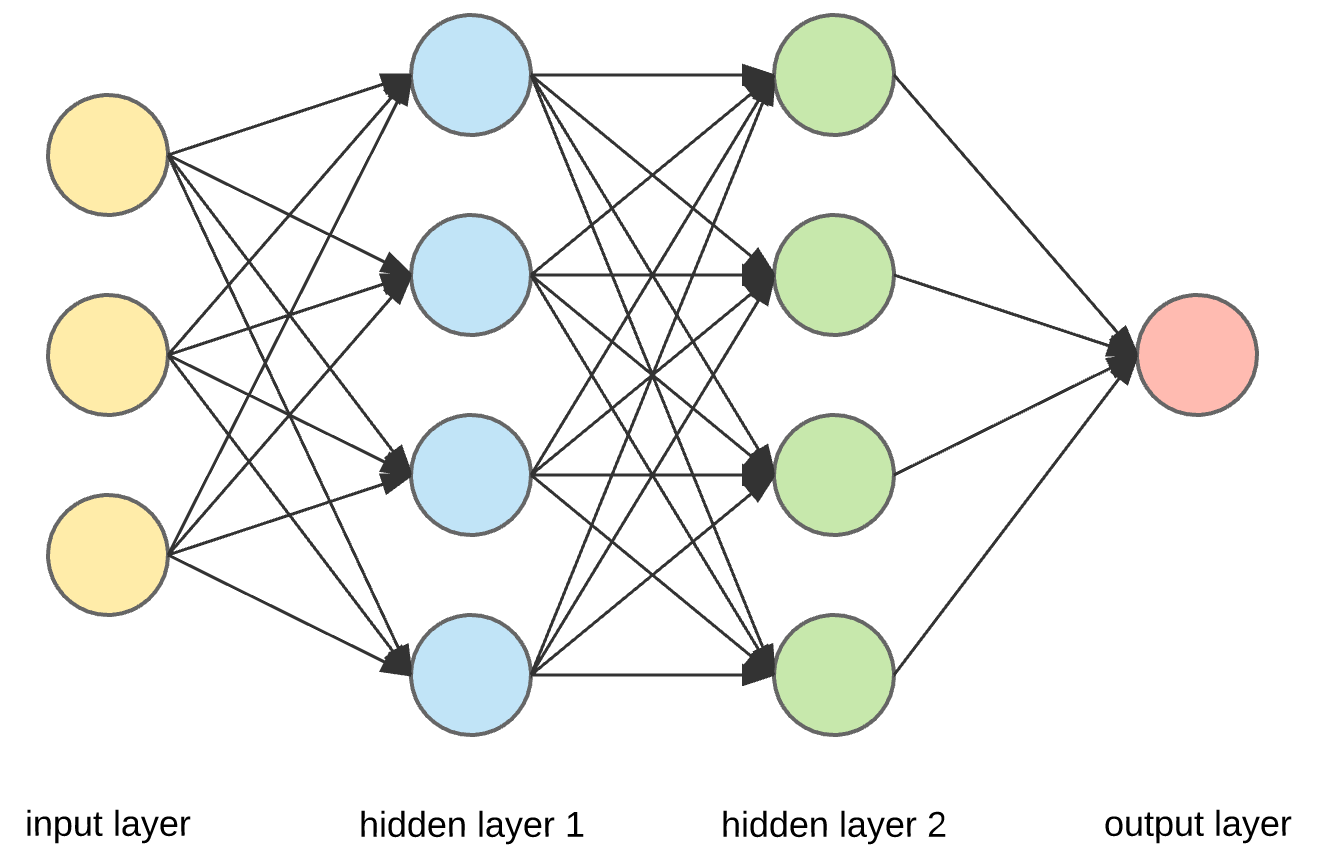
\includegraphics[width=0.38\linewidth]{dense_layer.png} 
    \caption{Potpuno povezani sloj}
    \label{slk:dense_layer}
\end{figure}

  \begin{equation}
    \label{jed:prvajednadzba}
    \int_{-\infty}^{+\infty}f(t)\,dt=F(\omega)
  \end{equation}


